\documentclass[mphy386-notes.tex]{subfiles}
\begin{document}
\section{X-Ray Image Quality}
In this section we will introduce the basics of x-ray imaging and develop three
tools that we can use to quantify image quality---contrast, resolution, and
noise. We will focus on x-ray imaging in these notes, but these tools are
useful for analyzing all imaging modalities.

\subsection{X-ray Imaging Basics}
We can create an x-ray imaging system by assembling an x-ray \textbf{source}, an
\textbf{object}, and a \textbf{detector}. Figure \ref{fig:simple} shows a simple
example of an x-ray imaging system---we place a constant x-ray fluence $\phi_0$
incident on an object with two attenuation coefficients $\mu_1$ and $\mu_2$.
\begin{figure}[h]
\begin{center}
  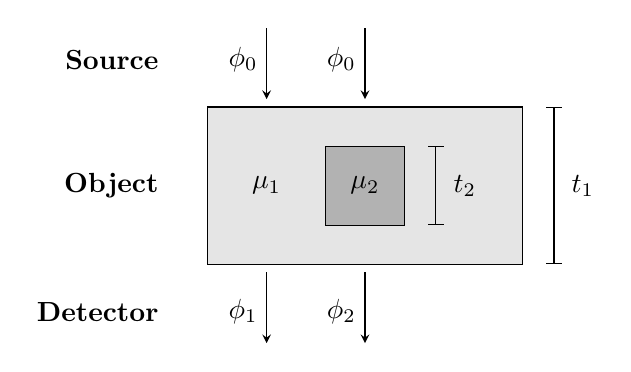
\begin{tikzpicture}[>=stealth]
    \filldraw[fill=black!10!white, draw=black] (-2,-1) rectangle (2,1);
    \filldraw[fill=black!30!white, draw=black] (-0.5,-0.5) rectangle (0.5,0.5);
    \draw [|-|] (2.4,-1) -- (2.4,1);
    \draw [|-|] (0.9,-0.5) -- (0.9,0.5);
    \node[right] at (1.0,0) {$t_2$};
    \node[right] at (2.5,0) {$t_1$};
    \node at (0,0) {$\mu_2$};
    \node at (-1.25,0) {$\mu_1$};
    \draw [->] (-1.25,2) -- (-1.25,1.1);
    \draw [->] (0,2) -- (0,1.1);
    \node at (-1.55,1.6) {$\phi_0$};
    \node at (-.3,1.6) {$\phi_0$};    
    \draw [->] (-1.25,-1.1) -- (-1.25,-2);
    \draw [->] (0,-1.1) -- (0,-2);
    \node at (-1.55,-1.6) {$\phi_1$};
    \node at (-.3,-1.6) {$\phi_2$};
    \node[left] at (-2.5, 1.6) {\textbf{Source}};
    \node[left] at (-2.5, 0) {\textbf{Object}};
    \node[left] at (-2.5, -1.6) {\textbf{Detector}};    
\end{tikzpicture}
\end{center}
\captionsetup{width=1.0\linewidth}
\caption{Simple x-ray imaging schematic.}
\label{fig:simple}
\end{figure}
X-rays are attenuated as they pass through the object so the fluences that
exit the object are related to the input fluence by
\begin{align}
  \phi_1 &= \phi_0e^{-\mu_1 t_1}\\
  \phi_2 &= \phi_0e^{-\mu_1(t_1 - t_2) - \mu_2t_2}. 
\end{align}
We measure the x-rays that exit the object with a detector and create an image.

We will examine more realistic sources and detectors in later sections, but the
simple example in Figure \ref{fig:simple} is sufficient for us to model image
quality in x-ray imaging systems. 

\subsection{Rose Model}
Suppose that we'd like to detect the presence or absence of the small object
with attenuation $\mu_2$ in Figure \ref{fig:simple} with our imaging system. How
well can we perform this task? What conditions do we need to meet to confidently
say that the object is present or absent? How should we design our imaging
system to meet these conditions? The Rose model supplies answers to these
questions and gives us a solid framework for understanding image quality.



The signal is the difference in intensity between the object and its background:
\begin{align*}
  \Delta S = S_1 - S_2 = A\phi_1 - A\phi_2 = A\Delta\phi.
\end{align*}
where $A$ is the cross sectional area of the object, $\phi$ is the x-ray fluence
with units of photons per unit area and $\Delta\phi = \phi_1-\phi_2$.

The noise is the square-root of the variance in background over areas the size
of the object. Assuming the noise follows Poisson statistics, where the
variance means the mean value
\begin{align}
  \text{Noise} = \sqrt{\sigma^2} = \sqrt{\frac{A\phi_1 + A\phi_2}{2}} = \sqrt{A\bar{\phi}}
\end{align}
Therefore, the signal-to-noise ratio is,
\begin{align}
  \text{SNR} &= \frac{A\Delta\phi}{\sqrt{A\bar{\phi}}}\\
  \text{SNR} &= C\sqrt{A\bar{\phi}} 
\end{align}
where $C$ is the radiation contrast:
\begin{align}
  C = \frac{\Delta\phi}{\bar{\phi}}
\end{align}
This is the SNR for an ideal detector where we've assumed that
\begin{itemize}
\item complete absorption of incident quanta
\item no added noise
\item no loss of spatial resolution (i.e., no blurring)
\end{itemize}

 \fig{img/rose.png}{.25}{Test}{rose}
 \fig{img/contrast.png}{.25}{Test}{constrast}

\pagebreak
\end{document}